\documentclass[]{article}
\usepackage{lmodern}
\usepackage{amssymb,amsmath}
\usepackage{ifxetex,ifluatex}
\usepackage{fixltx2e} % provides \textsubscript
\ifnum 0\ifxetex 1\fi\ifluatex 1\fi=0 % if pdftex
  \usepackage[T1]{fontenc}
  \usepackage[utf8]{inputenc}
\else % if luatex or xelatex
  \ifxetex
    \usepackage{mathspec}
  \else
    \usepackage{fontspec}
  \fi
  \defaultfontfeatures{Ligatures=TeX,Scale=MatchLowercase}
\fi
% use upquote if available, for straight quotes in verbatim environments
\IfFileExists{upquote.sty}{\usepackage{upquote}}{}
% use microtype if available
\IfFileExists{microtype.sty}{%
\usepackage[]{microtype}
\UseMicrotypeSet[protrusion]{basicmath} % disable protrusion for tt fonts
}{}
\PassOptionsToPackage{hyphens}{url} % url is loaded by hyperref
\usepackage[unicode=true]{hyperref}
\hypersetup{
            pdftitle={DATA 624 - PROJECT 2},
            pdfauthor={OMER OZEREN - GRACIE HAN},
            pdfborder={0 0 0},
            breaklinks=true}
\urlstyle{same}  % don't use monospace font for urls
\usepackage[margin=1in]{geometry}
\usepackage{color}
\usepackage{fancyvrb}
\newcommand{\VerbBar}{|}
\newcommand{\VERB}{\Verb[commandchars=\\\{\}]}
\DefineVerbatimEnvironment{Highlighting}{Verbatim}{commandchars=\\\{\}}
% Add ',fontsize=\small' for more characters per line
\usepackage{framed}
\definecolor{shadecolor}{RGB}{248,248,248}
\newenvironment{Shaded}{\begin{snugshade}}{\end{snugshade}}
\newcommand{\KeywordTok}[1]{\textcolor[rgb]{0.13,0.29,0.53}{\textbf{#1}}}
\newcommand{\DataTypeTok}[1]{\textcolor[rgb]{0.13,0.29,0.53}{#1}}
\newcommand{\DecValTok}[1]{\textcolor[rgb]{0.00,0.00,0.81}{#1}}
\newcommand{\BaseNTok}[1]{\textcolor[rgb]{0.00,0.00,0.81}{#1}}
\newcommand{\FloatTok}[1]{\textcolor[rgb]{0.00,0.00,0.81}{#1}}
\newcommand{\ConstantTok}[1]{\textcolor[rgb]{0.00,0.00,0.00}{#1}}
\newcommand{\CharTok}[1]{\textcolor[rgb]{0.31,0.60,0.02}{#1}}
\newcommand{\SpecialCharTok}[1]{\textcolor[rgb]{0.00,0.00,0.00}{#1}}
\newcommand{\StringTok}[1]{\textcolor[rgb]{0.31,0.60,0.02}{#1}}
\newcommand{\VerbatimStringTok}[1]{\textcolor[rgb]{0.31,0.60,0.02}{#1}}
\newcommand{\SpecialStringTok}[1]{\textcolor[rgb]{0.31,0.60,0.02}{#1}}
\newcommand{\ImportTok}[1]{#1}
\newcommand{\CommentTok}[1]{\textcolor[rgb]{0.56,0.35,0.01}{\textit{#1}}}
\newcommand{\DocumentationTok}[1]{\textcolor[rgb]{0.56,0.35,0.01}{\textbf{\textit{#1}}}}
\newcommand{\AnnotationTok}[1]{\textcolor[rgb]{0.56,0.35,0.01}{\textbf{\textit{#1}}}}
\newcommand{\CommentVarTok}[1]{\textcolor[rgb]{0.56,0.35,0.01}{\textbf{\textit{#1}}}}
\newcommand{\OtherTok}[1]{\textcolor[rgb]{0.56,0.35,0.01}{#1}}
\newcommand{\FunctionTok}[1]{\textcolor[rgb]{0.00,0.00,0.00}{#1}}
\newcommand{\VariableTok}[1]{\textcolor[rgb]{0.00,0.00,0.00}{#1}}
\newcommand{\ControlFlowTok}[1]{\textcolor[rgb]{0.13,0.29,0.53}{\textbf{#1}}}
\newcommand{\OperatorTok}[1]{\textcolor[rgb]{0.81,0.36,0.00}{\textbf{#1}}}
\newcommand{\BuiltInTok}[1]{#1}
\newcommand{\ExtensionTok}[1]{#1}
\newcommand{\PreprocessorTok}[1]{\textcolor[rgb]{0.56,0.35,0.01}{\textit{#1}}}
\newcommand{\AttributeTok}[1]{\textcolor[rgb]{0.77,0.63,0.00}{#1}}
\newcommand{\RegionMarkerTok}[1]{#1}
\newcommand{\InformationTok}[1]{\textcolor[rgb]{0.56,0.35,0.01}{\textbf{\textit{#1}}}}
\newcommand{\WarningTok}[1]{\textcolor[rgb]{0.56,0.35,0.01}{\textbf{\textit{#1}}}}
\newcommand{\AlertTok}[1]{\textcolor[rgb]{0.94,0.16,0.16}{#1}}
\newcommand{\ErrorTok}[1]{\textcolor[rgb]{0.64,0.00,0.00}{\textbf{#1}}}
\newcommand{\NormalTok}[1]{#1}
\usepackage{graphicx,grffile}
\makeatletter
\def\maxwidth{\ifdim\Gin@nat@width>\linewidth\linewidth\else\Gin@nat@width\fi}
\def\maxheight{\ifdim\Gin@nat@height>\textheight\textheight\else\Gin@nat@height\fi}
\makeatother
% Scale images if necessary, so that they will not overflow the page
% margins by default, and it is still possible to overwrite the defaults
% using explicit options in \includegraphics[width, height, ...]{}
\setkeys{Gin}{width=\maxwidth,height=\maxheight,keepaspectratio}
\IfFileExists{parskip.sty}{%
\usepackage{parskip}
}{% else
\setlength{\parindent}{0pt}
\setlength{\parskip}{6pt plus 2pt minus 1pt}
}
\setlength{\emergencystretch}{3em}  % prevent overfull lines
\providecommand{\tightlist}{%
  \setlength{\itemsep}{0pt}\setlength{\parskip}{0pt}}
\setcounter{secnumdepth}{0}
% Redefines (sub)paragraphs to behave more like sections
\ifx\paragraph\undefined\else
\let\oldparagraph\paragraph
\renewcommand{\paragraph}[1]{\oldparagraph{#1}\mbox{}}
\fi
\ifx\subparagraph\undefined\else
\let\oldsubparagraph\subparagraph
\renewcommand{\subparagraph}[1]{\oldsubparagraph{#1}\mbox{}}
\fi

% set default figure placement to htbp
\makeatletter
\def\fps@figure{htbp}
\makeatother

\usepackage{booktabs}
\usepackage{longtable}
\usepackage{array}
\usepackage{multirow}
\usepackage{wrapfig}
\usepackage{float}
\usepackage{colortbl}
\usepackage{pdflscape}
\usepackage{tabu}
\usepackage{threeparttable}
\usepackage{threeparttablex}
\usepackage[normalem]{ulem}
\usepackage{makecell}
\usepackage{xcolor}

\title{DATA 624 - PROJECT 2}
\author{OMER OZEREN - GRACIE HAN}
\date{}

\begin{document}
\maketitle

{
\setcounter{tocdepth}{3}
\tableofcontents
}
\section{Project 2}\label{project-2}

This is role playing. I am your new boss. I am in charge of production
at ABC Beverage and you are a team of data scientists reporting to me.
My leadership has told me that new regulations are requiring us to
understand our manufacturing process, the predictive factors and be able
to report to them our predictive model of PH.

Please use the historical data set I am providing. Build and report the
factors in BOTH a technical and non-technical report. I like to use Word
and Excel. Please provide your non-technical report in a business
friendly readable document and your predictions in an Excel readable
format. The technical report should show clearly the models you tested
and how you selected your final approach.

Please submit both Rpubs links and .rmd files or other readable formats
for technical and non-technical reports. Also submit the excel file
showing the prediction of your models for pH

\begin{Shaded}
\begin{Highlighting}[]
\KeywordTok{library}\NormalTok{(tidyverse)}
\KeywordTok{library}\NormalTok{(kableExtra)}
\KeywordTok{library}\NormalTok{(xgboost)}
\KeywordTok{library}\NormalTok{(plyr)}
\KeywordTok{library}\NormalTok{ (e1071)}
\KeywordTok{library}\NormalTok{(corrplot)}
\KeywordTok{library}\NormalTok{(ggplot2)}
\KeywordTok{library}\NormalTok{(tidyr)}
\KeywordTok{library}\NormalTok{(dplyr)}
\KeywordTok{library}\NormalTok{(caret)}
\KeywordTok{library}\NormalTok{(Matrix)}
\KeywordTok{library}\NormalTok{(writexl)}
\KeywordTok{library}\NormalTok{(psych)}
\end{Highlighting}
\end{Shaded}

\subsubsection{Load the Evaluation Data}\label{load-the-evaluation-data}

The data set contains 267 observations and 33 variables. The variable
name BrandCode is a character variable, the remaining variables are
numeric. PH is the respond variable

\subsubsection{Load the Train Data}\label{load-the-train-data}

\subsubsection{Train Data Statistics}\label{train-data-statistics}

\begin{verbatim}
## [1] 2571   33
\end{verbatim}

\subsubsection{Train Data Number of
Observations}\label{train-data-number-of-observations}

\begin{verbatim}
## [1] 2038
\end{verbatim}

\subsubsection{Train Data Summary}\label{train-data-summary}

\begin{verbatim}
##  Brand.Code   Carb.Volume     Fill.Ounces      PC.Volume       Carb.Pressure  
##  A   : 293   Min.   :5.040   Min.   :23.63   Min.   :0.07933   Min.   :57.00  
##  B   :1239   1st Qu.:5.293   1st Qu.:23.92   1st Qu.:0.23917   1st Qu.:65.60  
##  C   : 304   Median :5.347   Median :23.97   Median :0.27133   Median :68.20  
##  D   : 615   Mean   :5.370   Mean   :23.97   Mean   :0.27712   Mean   :68.19  
##  NA's: 120   3rd Qu.:5.453   3rd Qu.:24.03   3rd Qu.:0.31200   3rd Qu.:70.60  
##              Max.   :5.700   Max.   :24.32   Max.   :0.47800   Max.   :79.40  
##              NA's   :10      NA's   :38      NA's   :39        NA's   :27     
##    Carb.Temp          PSC             PSC.Fill         PSC.CO2       
##  Min.   :128.6   Min.   :0.00200   Min.   :0.0000   Min.   :0.00000  
##  1st Qu.:138.4   1st Qu.:0.04800   1st Qu.:0.1000   1st Qu.:0.02000  
##  Median :140.8   Median :0.07600   Median :0.1800   Median :0.04000  
##  Mean   :141.1   Mean   :0.08457   Mean   :0.1954   Mean   :0.05641  
##  3rd Qu.:143.8   3rd Qu.:0.11200   3rd Qu.:0.2600   3rd Qu.:0.08000  
##  Max.   :154.0   Max.   :0.27000   Max.   :0.6200   Max.   :0.24000  
##  NA's   :26      NA's   :33        NA's   :23       NA's   :39       
##     Mnf.Flow       Carb.Pressure1  Fill.Pressure   Hyd.Pressure1  
##  Min.   :-100.20   Min.   :105.6   Min.   :34.60   Min.   :-0.80  
##  1st Qu.:-100.00   1st Qu.:119.0   1st Qu.:46.00   1st Qu.: 0.00  
##  Median :  65.20   Median :123.2   Median :46.40   Median :11.40  
##  Mean   :  24.57   Mean   :122.6   Mean   :47.92   Mean   :12.44  
##  3rd Qu.: 140.80   3rd Qu.:125.4   3rd Qu.:50.00   3rd Qu.:20.20  
##  Max.   : 229.40   Max.   :140.2   Max.   :60.40   Max.   :58.00  
##  NA's   :2         NA's   :32      NA's   :22      NA's   :11     
##  Hyd.Pressure2   Hyd.Pressure3   Hyd.Pressure4     Filler.Level  
##  Min.   : 0.00   Min.   :-1.20   Min.   : 52.00   Min.   : 55.8  
##  1st Qu.: 0.00   1st Qu.: 0.00   1st Qu.: 86.00   1st Qu.: 98.3  
##  Median :28.60   Median :27.60   Median : 96.00   Median :118.4  
##  Mean   :20.96   Mean   :20.46   Mean   : 96.29   Mean   :109.3  
##  3rd Qu.:34.60   3rd Qu.:33.40   3rd Qu.:102.00   3rd Qu.:120.0  
##  Max.   :59.40   Max.   :50.00   Max.   :142.00   Max.   :161.2  
##  NA's   :15      NA's   :15      NA's   :30       NA's   :20     
##   Filler.Speed   Temperature      Usage.cont      Carb.Flow       Density     
##  Min.   : 998   Min.   :63.60   Min.   :12.08   Min.   :  26   Min.   :0.240  
##  1st Qu.:3888   1st Qu.:65.20   1st Qu.:18.36   1st Qu.:1144   1st Qu.:0.900  
##  Median :3982   Median :65.60   Median :21.79   Median :3028   Median :0.980  
##  Mean   :3687   Mean   :65.97   Mean   :20.99   Mean   :2468   Mean   :1.174  
##  3rd Qu.:3998   3rd Qu.:66.40   3rd Qu.:23.75   3rd Qu.:3186   3rd Qu.:1.620  
##  Max.   :4030   Max.   :76.20   Max.   :25.90   Max.   :5104   Max.   :1.920  
##  NA's   :57     NA's   :14      NA's   :5       NA's   :2      NA's   :1      
##       MFR           Balling       Pressure.Vacuum        PH       
##  Min.   : 31.4   Min.   :-0.170   Min.   :-6.600   Min.   :7.880  
##  1st Qu.:706.3   1st Qu.: 1.496   1st Qu.:-5.600   1st Qu.:8.440  
##  Median :724.0   Median : 1.648   Median :-5.400   Median :8.540  
##  Mean   :704.0   Mean   : 2.198   Mean   :-5.216   Mean   :8.546  
##  3rd Qu.:731.0   3rd Qu.: 3.292   3rd Qu.:-5.000   3rd Qu.:8.680  
##  Max.   :868.6   Max.   : 4.012   Max.   :-3.600   Max.   :9.360  
##  NA's   :212     NA's   :1                         NA's   :4      
##  Oxygen.Filler     Bowl.Setpoint   Pressure.Setpoint Air.Pressurer  
##  Min.   :0.00240   Min.   : 70.0   Min.   :44.00     Min.   :140.8  
##  1st Qu.:0.02200   1st Qu.:100.0   1st Qu.:46.00     1st Qu.:142.2  
##  Median :0.03340   Median :120.0   Median :46.00     Median :142.6  
##  Mean   :0.04684   Mean   :109.3   Mean   :47.62     Mean   :142.8  
##  3rd Qu.:0.06000   3rd Qu.:120.0   3rd Qu.:50.00     3rd Qu.:143.0  
##  Max.   :0.40000   Max.   :140.0   Max.   :52.00     Max.   :148.2  
##  NA's   :12        NA's   :2       NA's   :12                       
##     Alch.Rel        Carb.Rel      Balling.Lvl  
##  Min.   :5.280   Min.   :4.960   Min.   :0.00  
##  1st Qu.:6.540   1st Qu.:5.340   1st Qu.:1.38  
##  Median :6.560   Median :5.400   Median :1.48  
##  Mean   :6.897   Mean   :5.437   Mean   :2.05  
##  3rd Qu.:7.240   3rd Qu.:5.540   3rd Qu.:3.14  
##  Max.   :8.620   Max.   :6.060   Max.   :3.66  
##  NA's   :9       NA's   :10      NA's   :1
\end{verbatim}

The training data set contains 2571 observations and 33 variables. The
variable name BrandCode is a character variable, the remaining variables
are numeric. PH is the response variable.

\subsubsection{Summary Statistics of Train
Data}\label{summary-statistics-of-train-data}

\begin{table}

\caption{\label{tab:unnamed-chunk-5}Descriptive Statistics for Train Data}
\centering
\begin{tabular}[t]{l|r|r|r|r|r|r|r|r|r}
\hline
  & n & mean & sd & median & min & max & range & skew & kurtosis\\
\hline
Brand.Code* & 2451 & 2.51 & 1.00 & 2.00 & 1.00 & 4.00 & 3.00 & 0.38 & -1.06\\
\hline
Carb.Volume & 2561 & 5.37 & 0.11 & 5.35 & 5.04 & 5.70 & 0.66 & 0.39 & -0.47\\
\hline
Fill.Ounces & 2533 & 23.97 & 0.09 & 23.97 & 23.63 & 24.32 & 0.69 & -0.02 & 0.86\\
\hline
PC.Volume & 2532 & 0.28 & 0.06 & 0.27 & 0.08 & 0.48 & 0.40 & 0.34 & 0.67\\
\hline
Carb.Pressure & 2544 & 68.19 & 3.54 & 68.20 & 57.00 & 79.40 & 22.40 & 0.18 & -0.01\\
\hline
Carb.Temp & 2545 & 141.09 & 4.04 & 140.80 & 128.60 & 154.00 & 25.40 & 0.25 & 0.24\\
\hline
PSC & 2538 & 0.08 & 0.05 & 0.08 & 0.00 & 0.27 & 0.27 & 0.85 & 0.65\\
\hline
PSC.Fill & 2548 & 0.20 & 0.12 & 0.18 & 0.00 & 0.62 & 0.62 & 0.93 & 0.77\\
\hline
PSC.CO2 & 2532 & 0.06 & 0.04 & 0.04 & 0.00 & 0.24 & 0.24 & 1.73 & 3.73\\
\hline
Mnf.Flow & 2569 & 24.57 & 119.48 & 65.20 & -100.20 & 229.40 & 329.60 & 0.00 & -1.87\\
\hline
Carb.Pressure1 & 2539 & 122.59 & 4.74 & 123.20 & 105.60 & 140.20 & 34.60 & 0.05 & 0.14\\
\hline
Fill.Pressure & 2549 & 47.92 & 3.18 & 46.40 & 34.60 & 60.40 & 25.80 & 0.55 & 1.41\\
\hline
Hyd.Pressure1 & 2560 & 12.44 & 12.43 & 11.40 & -0.80 & 58.00 & 58.80 & 0.78 & -0.14\\
\hline
Hyd.Pressure2 & 2556 & 20.96 & 16.39 & 28.60 & 0.00 & 59.40 & 59.40 & -0.30 & -1.56\\
\hline
Hyd.Pressure3 & 2556 & 20.46 & 15.98 & 27.60 & -1.20 & 50.00 & 51.20 & -0.32 & -1.57\\
\hline
Hyd.Pressure4 & 2541 & 96.29 & 13.12 & 96.00 & 52.00 & 142.00 & 90.00 & 0.55 & 0.63\\
\hline
Filler.Level & 2551 & 109.25 & 15.70 & 118.40 & 55.80 & 161.20 & 105.40 & -0.85 & 0.05\\
\hline
Filler.Speed & 2514 & 3687.20 & 770.82 & 3982.00 & 998.00 & 4030.00 & 3032.00 & -2.87 & 6.71\\
\hline
Temperature & 2557 & 65.97 & 1.38 & 65.60 & 63.60 & 76.20 & 12.60 & 2.39 & 10.16\\
\hline
Usage.cont & 2566 & 20.99 & 2.98 & 21.79 & 12.08 & 25.90 & 13.82 & -0.54 & -1.02\\
\hline
Carb.Flow & 2569 & 2468.35 & 1073.70 & 3028.00 & 26.00 & 5104.00 & 5078.00 & -0.99 & -0.58\\
\hline
Density & 2570 & 1.17 & 0.38 & 0.98 & 0.24 & 1.92 & 1.68 & 0.53 & -1.20\\
\hline
MFR & 2359 & 704.05 & 73.90 & 724.00 & 31.40 & 868.60 & 837.20 & -5.09 & 30.46\\
\hline
Balling & 2570 & 2.20 & 0.93 & 1.65 & -0.17 & 4.01 & 4.18 & 0.59 & -1.39\\
\hline
Pressure.Vacuum & 2571 & -5.22 & 0.57 & -5.40 & -6.60 & -3.60 & 3.00 & 0.53 & -0.03\\
\hline
PH & 2567 & 8.55 & 0.17 & 8.54 & 7.88 & 9.36 & 1.48 & -0.29 & 0.06\\
\hline
Oxygen.Filler & 2559 & 0.05 & 0.05 & 0.03 & 0.00 & 0.40 & 0.40 & 2.66 & 11.09\\
\hline
Bowl.Setpoint & 2569 & 109.33 & 15.30 & 120.00 & 70.00 & 140.00 & 70.00 & -0.97 & -0.06\\
\hline
Pressure.Setpoint & 2559 & 47.62 & 2.04 & 46.00 & 44.00 & 52.00 & 8.00 & 0.20 & -1.60\\
\hline
Air.Pressurer & 2571 & 142.83 & 1.21 & 142.60 & 140.80 & 148.20 & 7.40 & 2.25 & 4.73\\
\hline
Alch.Rel & 2562 & 6.90 & 0.51 & 6.56 & 5.28 & 8.62 & 3.34 & 0.88 & -0.85\\
\hline
Carb.Rel & 2561 & 5.44 & 0.13 & 5.40 & 4.96 & 6.06 & 1.10 & 0.50 & -0.29\\
\hline
Balling.Lvl & 2570 & 2.05 & 0.87 & 1.48 & 0.00 & 3.66 & 3.66 & 0.59 & -1.49\\
\hline
\end{tabular}
\end{table}

There are 2038 observations that has no missing values in any of the 33
columns, which indicates that the data has minimum missing values. It
also means that there are 533 (2571 minus 2038) observations that has
some missing values in some of their variables.

Looking at Missing values of each of the numerical variables, the
maximum NA is 212 at MFR ,followed by Filler Speed (57 missing),
followed by a few variables which has missing values in 30s (PC volume,
fill ounces, PSC CO2, carb pressure 1, hyd pressure 4), then Followed by
variables which has missing values in 20s (carb pressure, PSC Phil, feel
pressure, filler level). Then, the rest of the variables Have missing
values that are in teens or below.

Kurtosis For each of the variables also confirmed that MFR is highly
skilled with Kurtosis=30.46. Mnf Flow have a median at 724, and mean at
704. But the range of it is from 31.4 till 868, with a wopping range of
837!

Besides MFR, the skewness of the rest of the variables are alright. The
next batch of variables with relatively high skewness (their Kurtosis
value) is temperature ( endpoint one 6 ), oxygen filler ( 11.09 ), and
air pressure ( 4.73 ) .

\paragraph{Visualization of Target Variable
(pH)}\label{visualization-of-target-variable-ph}

\begin{center}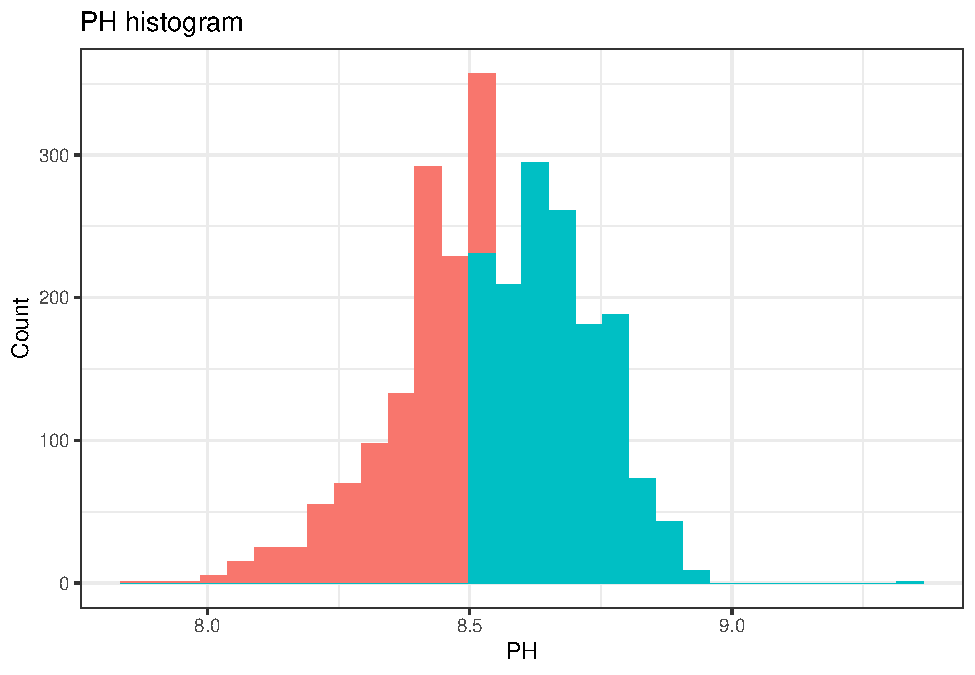
\includegraphics{OmerOzeren_GracieHan_Project_2_files/figure-latex/unnamed-chunk-6-1} \end{center}

The outcome variable, PH value in the beverage, is shown on histogram
here. We can see that it is a continuous variable with no gap at no
clear patterns of missing value.

Except a few observations which is somewhat outliers at the right tale,
it pretty much follows a normal distribution. There are slightly more
observations on the right side ( higher values ) of the histogram, but
we decide not to do too much about it because the s Skewness is minimum.

We decided that this outcome is satisfactory in being used as is as a
numerical variable outcome. We will provide models based on PH outcome
as a continuous numerical variable, without intentional cutoff points
below.

\subsubsection{Visualization of
Predictors}\label{visualization-of-predictors}

\begin{center}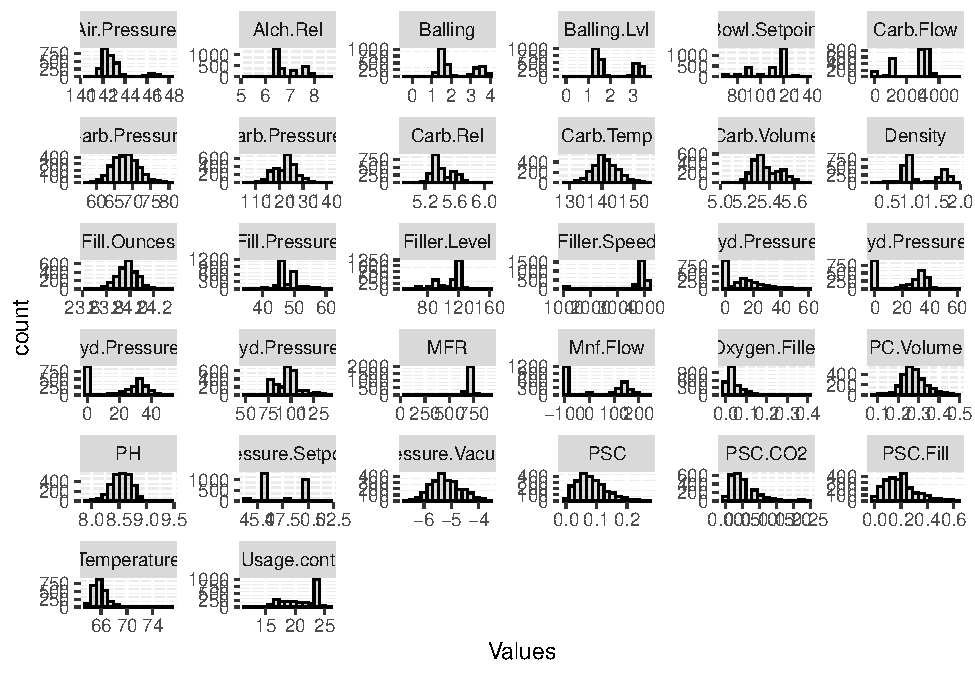
\includegraphics{OmerOzeren_GracieHan_Project_2_files/figure-latex/unnamed-chunk-7-1} \end{center}

Visualization of histogram of each individual predictor variables
indicate that beside the numerical variables, there are many categorical
variables (discrete variables), such as pressure.set point, aich.rel).

The obvious discrete variables are: Brand Code (ABCD 4 brands in total),
Pressure Setpoint, Bowl Setpoint, PSC.CO2, Pressure Vacuume. Each of
these varaiables have no more than 10-12 unique numbers to make the
count.

There are some bi-mode variables: (such as pressure set point, density,
hyd pressure 2, hyd pressure3).\\
Multi-mode (\textgreater{}2mode) Variables include carb flow.

Histogram also indicated the right skewness of MFR, which has a spike of
counts at around the 40.

These variables have a significant numbers of apps observations at 0:
hyd pressure1,hyd pressure2,hyd pressure 3,

The close to normally distributed variables judging from the histograms
are : carb pressure 1, carb pressure 2, Carb Temp, Carb Volume, Fill
Ounces, PC Volume.

We chose bins=15 and facet wrap for the histograms. This findings are
preserved after changing the numbers of bins.

\subsubsection{Outliers Analysis with
Boxplot}\label{outliers-analysis-with-boxplot}

\begin{center}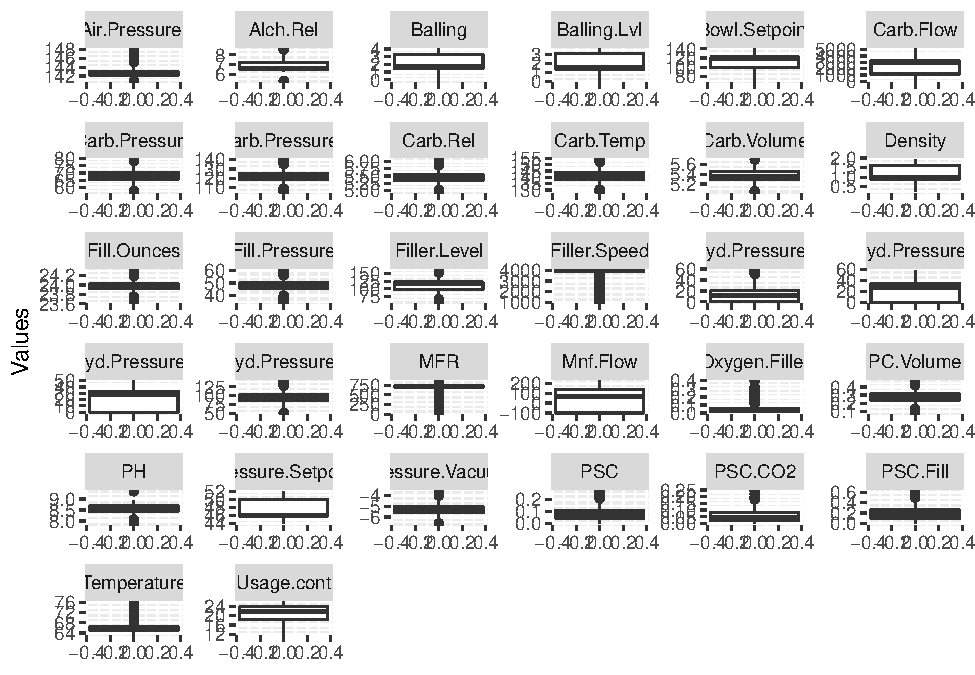
\includegraphics{OmerOzeren_GracieHan_Project_2_files/figure-latex/unnamed-chunk-8-1} \end{center}

Because some of the variables are skewed, so the box plot shows data
many of these predictors are recognized as outliers. these variables
include: MFR ,filler.speed, Oxygen,filler, Air.presseurer. But we
predict that after transformation later on, some of these so called
``outliers'' will not persist.

Besides the above mentioned four variables, these variables also have
extreme outliers: PSC fill, PSC CO2, Temperature, Pressure.vacume,
Alch.Rel, Carb.Rel.

Interestingly, the outcome variable pH also have a few outliers.

\subsubsection{Relationships Between the Target and Explanatory
Variables}\label{relationships-between-the-target-and-explanatory-variables}

This plot below indicates relationship between target and explanatory
variables

\begin{center}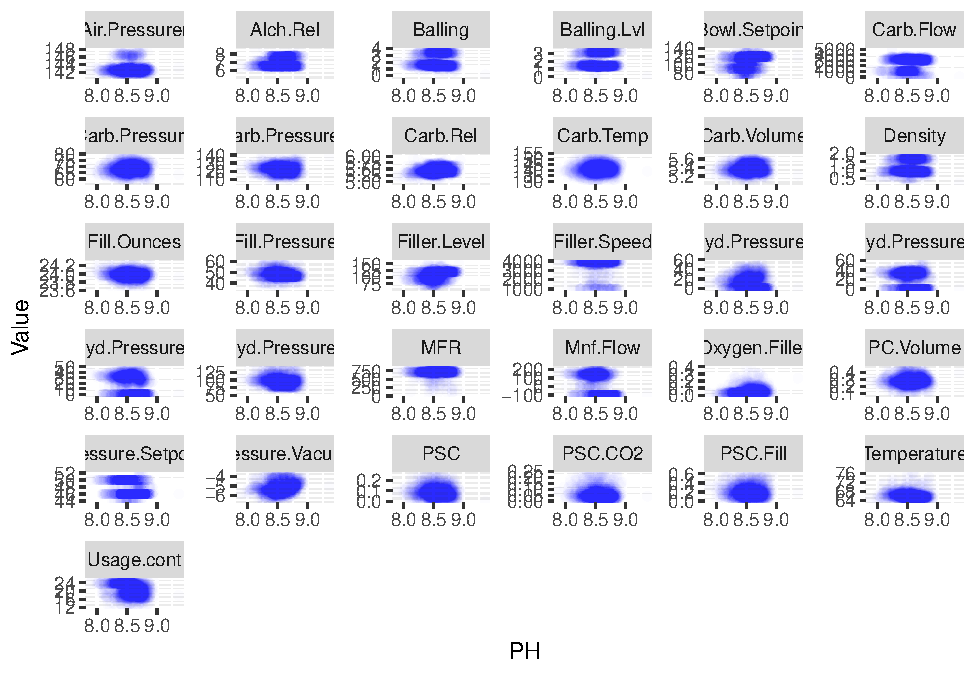
\includegraphics{OmerOzeren_GracieHan_Project_2_files/figure-latex/unnamed-chunk-9-1} \end{center}

Among all 33 predicted variables my, majority of them have clear
Association with the outcome. Maybe half of these predictors, if they
are numerical and continuous, have clear relationship to the outcome in
linear fashion. The predictors that clear Le demonstrate the linearity
with the outcome include below:

Carb volume, fill ounces, PC volumes, carb pressure, carb temperatures,
PSC fill, PSC, carb pressure1, carb rel.

Explaining these variables from common sense perspective, they all make
sense in beverage production, we feel that these variables are the
predictors that have good and continuous measurement, oftentimes from
the environment, rather than work worker controlled source. Therefore,
it is not surprising that they have good linearity with the pH value
(outcome) of the beverage.

Above is the good news from predictors, which favors linear model, as
well as other tree based the models. However, we have also seen that
many other variables, even that they are linear and numerical
predictors, they either have outliers, or their measure month is not
continuous enough, in other words, interrupted in patterns, therefore
may produce errors if we fit the linear model two outcome directly
without tuning of these variables, or without other sophisticated
modeling. Such non perfect numerical predictor variables include:

Mnf Flow, fill pressure, Hyd pressure 1, Hyd Pressure2, Hyd pressure3,
Fill levels, Filler Speed, temperature, carb flow, MFR, Density,
Bailing, Oxygen Filler, Air Pressure

Finally many of the predictor variables are in discrete or nominal
variable fashion, which has levels in less than 10 or even 3. so when we
fit these variables into the model, we have to be oh extremely careful
that the levels of predictors can be overly simplified in terms of
explanation due to the overly crude way of describing the nature of this
variable.

\subsubsection{Correlation}\label{correlation}

\begin{center}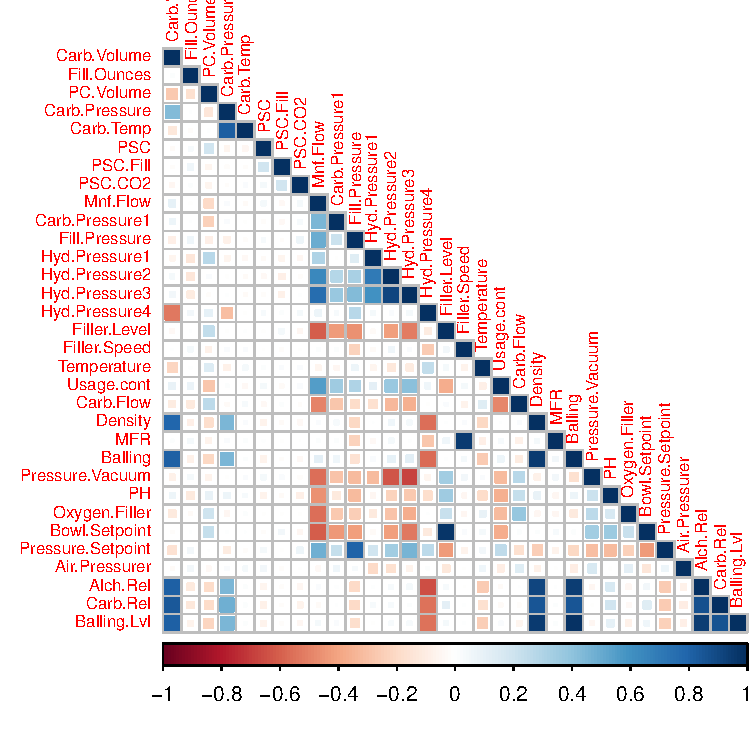
\includegraphics{OmerOzeren_GracieHan_Project_2_files/figure-latex/corrgram-1} \end{center}

We find the following very strong correlations: Carb.Volume with
Density, Balling, Alch.Rel, Carb.Rel, and Balling.Lvl.

Carb.Pressure with Carb.Temp Filler.Level with Bowl.Setpoint
Filler.Speed with MFR

Correlation plot above indicates that some explanantory variables are
correleted each other.

We find out explanantory variables that hig correleted each other by
using findCorrelation() with using threshold as 0.6.

\begin{verbatim}
##  [1] "Mnf.Flow"      "Balling"       "Hyd.Pressure3" "Alch.Rel"     
##  [5] "Balling.Lvl"   "Carb.Rel"      "Density"       "Hyd.Pressure2"
##  [9] "Fill.Pressure" "Filler.Level"  "Carb.Pressure" "Filler.Speed"
\end{verbatim}

Below shows top 10 Explanatory variables that positively correleted
highly to PH

\begin{verbatim}
##            rowname         PH
## 1               PH 1.00000000
## 2    Bowl.Setpoint 0.36158753
## 3     Filler.Level 0.35204396
## 4        Carb.Flow 0.23359370
## 5  Pressure.Vacuum 0.21973550
## 6         Carb.Rel 0.19605148
## 7         Alch.Rel 0.16668223
## 8    Oxygen.Filler 0.16448536
## 9      Balling.Lvl 0.10937117
## 10       PC.Volume 0.09886673
\end{verbatim}

Bowl Setpoint, Filler Level, Carb Flow, Pressure Vacuum are the top 5
explanatory variables that are positively associated with the PH
outcome.

Their correlation to the PH outcome rANGES FROM 0.36 (TOP1) TO 0.22 (TOP
5TH).

The next set of varialbes (top 6-top10) have a correlation to outcome
range from 0.196 (top 6th) to 0.098 (top 10th).

Below shows top 10 Explanatory variables that negatively correlated
highly to PH

\begin{verbatim}
##              rowname         PH
## 1           Mnf.Flow -0.4592313
## 2         Usage.cont -0.3576120
## 3      Fill.Pressure -0.3165145
## 4  Pressure.Setpoint -0.3116639
## 5      Hyd.Pressure3 -0.2681018
## 6      Hyd.Pressure2 -0.2226600
## 7        Temperature -0.1826596
## 8      Hyd.Pressure4 -0.1714340
## 9     Carb.Pressure1 -0.1187642
## 10       Fill.Ounces -0.1183359
\end{verbatim}

Mnf Flow stands out as the top 1 variable that is negatively associated
with the PH outcome (correlation = -0.46), with a much higher
correlation than the 2nd variable Usage Count (correlation at -0.35).

Also, Fill Pressure, PRessure Setpoint have a correlation with PH around
-0.35.

\subsubsection{Near Zero Variance
Predictors}\label{near-zero-variance-predictors}

\begin{verbatim}
## NULL
\end{verbatim}

``Hyd Pressure1'' should be removed from the dataset since it hold
constant values.WE are going to handle this in Model Data PreProcessing
part

\subsubsection{Missing Values}\label{missing-values}

Using VIM library to explore missing values.

\begin{center}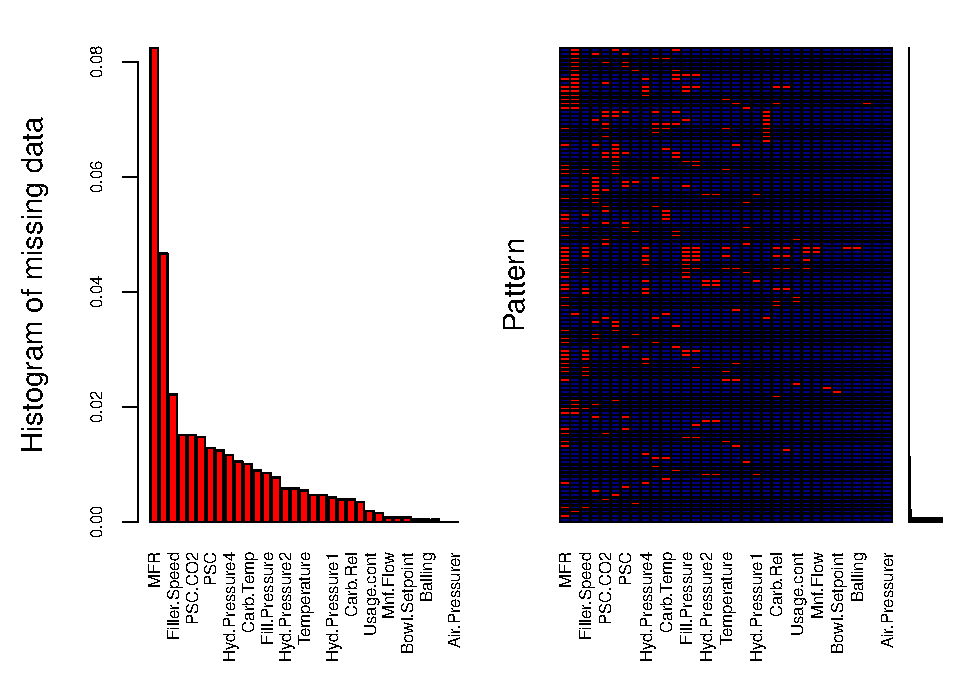
\includegraphics{OmerOzeren_GracieHan_Project_2_files/figure-latex/unnamed-chunk-14-1} \end{center}

\begin{verbatim}
## 
##  Variables sorted by number of missings: 
##           Variable        Count
##                MFR 0.0824581875
##         Brand.Code 0.0466744457
##       Filler.Speed 0.0221703617
##          PC.Volume 0.0151691949
##            PSC.CO2 0.0151691949
##        Fill.Ounces 0.0147802412
##                PSC 0.0128354726
##     Carb.Pressure1 0.0124465189
##      Hyd.Pressure4 0.0116686114
##      Carb.Pressure 0.0105017503
##          Carb.Temp 0.0101127966
##           PSC.Fill 0.0089459354
##      Fill.Pressure 0.0085569817
##       Filler.Level 0.0077790743
##      Hyd.Pressure2 0.0058343057
##      Hyd.Pressure3 0.0058343057
##        Temperature 0.0054453520
##      Oxygen.Filler 0.0046674446
##  Pressure.Setpoint 0.0046674446
##      Hyd.Pressure1 0.0042784909
##        Carb.Volume 0.0038895371
##           Carb.Rel 0.0038895371
##           Alch.Rel 0.0035005834
##         Usage.cont 0.0019447686
##                 PH 0.0015558149
##           Mnf.Flow 0.0007779074
##          Carb.Flow 0.0007779074
##      Bowl.Setpoint 0.0007779074
##            Density 0.0003889537
##            Balling 0.0003889537
##        Balling.Lvl 0.0003889537
##    Pressure.Vacuum 0.0000000000
##      Air.Pressurer 0.0000000000
\end{verbatim}

MFR stands out as a Having a significant amount of missings.

Followed by fillet speed, pace co2.

These three variables contains as many missing values as the rest of all
missing values from all variables.

The pattern of MR indicates that it has more missing values at the high
end, and the also in the middle part.

\subsection{Modeling Data
PreProcessing}\label{modeling-data-preprocessing}

\begin{verbatim}
##  Brand.Code  Carb.Volume     Fill.Ounces      PC.Volume       Carb.Pressure  
##  A: 305     Min.   :5.040   Min.   :23.63   Min.   :0.07933   Min.   :57.00  
##  B:1312     1st Qu.:5.293   1st Qu.:23.92   1st Qu.:0.23933   1st Qu.:65.60  
##  C: 333     Median :5.347   Median :23.97   Median :0.27133   Median :68.20  
##  D: 621     Mean   :5.370   Mean   :23.97   Mean   :0.27781   Mean   :68.22  
##             3rd Qu.:5.453   3rd Qu.:24.03   3rd Qu.:0.31267   3rd Qu.:70.60  
##             Max.   :5.700   Max.   :24.32   Max.   :0.47800   Max.   :79.40  
##    Carb.Temp          PSC           PSC.Fill         PSC.CO2       
##  Min.   :128.6   Min.   :0.002   Min.   :0.0000   Min.   :0.00000  
##  1st Qu.:138.4   1st Qu.:0.048   1st Qu.:0.1000   1st Qu.:0.02000  
##  Median :140.8   Median :0.078   Median :0.1800   Median :0.04000  
##  Mean   :141.1   Mean   :0.085   Mean   :0.1958   Mean   :0.05644  
##  3rd Qu.:143.8   3rd Qu.:0.112   3rd Qu.:0.2600   3rd Qu.:0.08000  
##  Max.   :154.0   Max.   :0.270   Max.   :0.6200   Max.   :0.24000  
##     Mnf.Flow       Carb.Pressure1  Fill.Pressure   Hyd.Pressure2  
##  Min.   :-100.20   Min.   :105.6   Min.   :34.60   Min.   : 0.00  
##  1st Qu.:-100.00   1st Qu.:118.8   1st Qu.:46.00   1st Qu.: 0.00  
##  Median :  64.80   Median :123.2   Median :46.40   Median :28.60  
##  Mean   :  24.47   Mean   :122.5   Mean   :47.92   Mean   :20.97  
##  3rd Qu.: 140.80   3rd Qu.:125.4   3rd Qu.:50.00   3rd Qu.:34.60  
##  Max.   : 229.40   Max.   :140.2   Max.   :60.40   Max.   :59.40  
##  Hyd.Pressure3   Hyd.Pressure4     Filler.Level    Filler.Speed 
##  Min.   :-1.20   Min.   : 52.00   Min.   : 55.8   Min.   : 998  
##  1st Qu.: 0.00   1st Qu.: 86.00   1st Qu.: 97.7   1st Qu.:3819  
##  Median :27.60   Median : 96.00   Median :118.4   Median :3980  
##  Mean   :20.44   Mean   : 96.53   Mean   :109.2   Mean   :3637  
##  3rd Qu.:33.20   3rd Qu.:102.00   3rd Qu.:120.0   3rd Qu.:3996  
##  Max.   :50.00   Max.   :142.00   Max.   :161.2   Max.   :4030  
##   Temperature      Usage.cont      Carb.Flow       Density           MFR       
##  Min.   :63.60   Min.   :12.08   Min.   :  26   Min.   :0.240   Min.   : 31.4  
##  1st Qu.:65.20   1st Qu.:18.36   1st Qu.:1142   1st Qu.:0.900   1st Qu.:695.0  
##  Median :65.60   Median :21.78   Median :3028   Median :0.980   Median :721.4  
##  Mean   :65.98   Mean   :20.99   Mean   :2468   Mean   :1.174   Mean   :669.8  
##  3rd Qu.:66.40   3rd Qu.:23.75   3rd Qu.:3186   3rd Qu.:1.620   3rd Qu.:730.4  
##  Max.   :76.20   Max.   :25.90   Max.   :5104   Max.   :1.920   Max.   :868.6  
##     Balling       Pressure.Vacuum        PH        Oxygen.Filler    
##  Min.   :-0.170   Min.   :-6.600   Min.   :7.880   Min.   :0.00240  
##  1st Qu.: 1.496   1st Qu.:-5.600   1st Qu.:8.440   1st Qu.:0.02200  
##  Median : 1.648   Median :-5.400   Median :8.540   Median :0.03340  
##  Mean   : 2.198   Mean   :-5.216   Mean   :8.546   Mean   :0.04712  
##  3rd Qu.: 3.292   3rd Qu.:-5.000   3rd Qu.:8.680   3rd Qu.:0.06000  
##  Max.   : 4.012   Max.   :-3.600   Max.   :9.360   Max.   :0.40000  
##  Bowl.Setpoint   Pressure.Setpoint Air.Pressurer      Alch.Rel    
##  Min.   : 70.0   Min.   :44.00     Min.   :140.8   Min.   :5.280  
##  1st Qu.:100.0   1st Qu.:46.00     1st Qu.:142.2   1st Qu.:6.540  
##  Median :120.0   Median :46.00     Median :142.6   Median :6.560  
##  Mean   :109.3   Mean   :47.61     Mean   :142.8   Mean   :6.897  
##  3rd Qu.:120.0   3rd Qu.:50.00     3rd Qu.:143.0   3rd Qu.:7.240  
##  Max.   :140.0   Max.   :52.00     Max.   :148.2   Max.   :8.620  
##     Carb.Rel      Balling.Lvl  
##  Min.   :4.960   Min.   :0.00  
##  1st Qu.:5.340   1st Qu.:1.38  
##  Median :5.400   Median :1.48  
##  Mean   :5.436   Mean   :2.05  
##  3rd Qu.:5.540   3rd Qu.:3.14  
##  Max.   :6.060   Max.   :3.66
\end{verbatim}

We used MICE package, CMM method to impute the missing data.

For the variables that has near zero observations, we used the function
of nearzeroVar, to avoid imputing the missing zeros.

From previous data exploration, we know that the non-zero observations
occur most in the variables of HYD pressure1.

By choosing not to impute the variable of HYD pressure1 (with non
zeros), in the evaluated model, we exclude that variable.

let's look at the variables missing percentage after impution to check
if we missing anything.

\begin{center}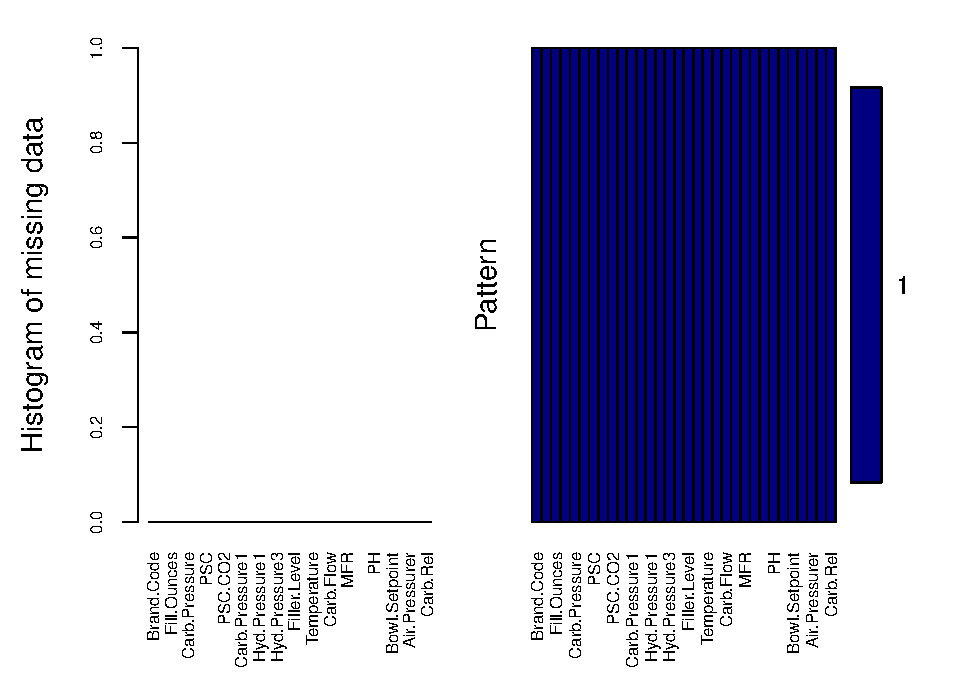
\includegraphics{OmerOzeren_GracieHan_Project_2_files/figure-latex/unnamed-chunk-15-1} \end{center}

\begin{verbatim}
## 
##  Variables sorted by number of missings: 
##           Variable Count
##         Brand.Code     0
##        Carb.Volume     0
##        Fill.Ounces     0
##          PC.Volume     0
##      Carb.Pressure     0
##          Carb.Temp     0
##                PSC     0
##           PSC.Fill     0
##            PSC.CO2     0
##           Mnf.Flow     0
##     Carb.Pressure1     0
##      Fill.Pressure     0
##      Hyd.Pressure1     0
##      Hyd.Pressure2     0
##      Hyd.Pressure3     0
##      Hyd.Pressure4     0
##       Filler.Level     0
##       Filler.Speed     0
##        Temperature     0
##         Usage.cont     0
##          Carb.Flow     0
##            Density     0
##                MFR     0
##            Balling     0
##    Pressure.Vacuum     0
##                 PH     0
##      Oxygen.Filler     0
##      Bowl.Setpoint     0
##  Pressure.Setpoint     0
##      Air.Pressurer     0
##           Alch.Rel     0
##           Carb.Rel     0
\end{verbatim}

By using the aggr function, we visualized the missing variables again.

We can see that on the left side graph, there is no missing values from
the data anymore. On the right side, the figure shows that all the
missing variables are now complete.

This figure (on the right side) also showed us that there is one
variable that this amputation has excluded, due to our command to
exclude the near zero variable, and as we know, this variable is HYD
pressure1. Now the data is good for furthe analysis.

\subsubsection{Splitting Data Set}\label{splitting-data-set}

Splitting dataset into training and test sets.

We used the 80/20 rule to create the training data set and the testing
data set. The function of createDataPartition is used for that purpose,
which select the random sample from the completed Data. Here, completed
means imputed data.

\subsection{Model Building \&
Evaluation}\label{model-building-evaluation}

Now the Data has been evaluated, with missing that is imputed. The Data
is ready to go for various of Modeling effort.

First,before any modeling occured, we created an empty data frame called
models\_test\_evaluation, which is the place holder for all the model
evaluates. For each model, we will select Root Mean Square of Error
(RMSE), R-squared, Mean Aboslute Error (MAE). Once these evaluators are
available from the model run, they are put into this dataframe, one row
per modeling.

We first will run the traditional linear regression model, as we have
numerical outcome, and mostly numerical predictors.

Next we will apply a few of the tree-based model and rule based models,
which are more modern, and utilizing the 33 variables in an ensumble (or
bagged way/mechanism), rather than assuming all linearity relationship
to the outcome for all 33 predictor variables indiviually, Which as we
know is a very strict assumption, and our data does not fully support
that assumption.

Most of the variables are associated with outcome, but not in the linear
fashion.

\subsubsection{Linear Regression Model}\label{linear-regression-model}

\begin{verbatim}
## 
## Call:
## lm(formula = PH ~ ., data = train_data)
## 
## Residuals:
##      Min       1Q   Median       3Q      Max 
## -0.51863 -0.07572  0.01150  0.08913  0.85621 
## 
## Coefficients:
##                     Estimate Std. Error t value Pr(>|t|)    
## (Intercept)        1.028e+01  1.180e+00   8.714  < 2e-16 ***
## Brand.CodeB        3.533e-02  2.215e-02   1.595 0.110876    
## Brand.CodeC       -8.893e-02  2.212e-02  -4.020 6.03e-05 ***
## Brand.CodeD        6.722e-02  1.821e-02   3.692 0.000228 ***
## Carb.Volume       -5.349e-02  1.001e-01  -0.535 0.593019    
## Fill.Ounces       -6.645e-02  3.542e-02  -1.876 0.060798 .  
## PC.Volume         -1.056e-01  5.824e-02  -1.813 0.069929 .  
## Carb.Pressure     -5.154e-04  4.680e-03  -0.110 0.912319    
## Carb.Temp          1.645e-03  3.707e-03   0.444 0.657278    
## PSC               -1.262e-01  6.481e-02  -1.948 0.051597 .  
## PSC.Fill          -4.041e-02  2.621e-02  -1.542 0.123253    
## PSC.CO2           -1.537e-01  7.024e-02  -2.189 0.028745 *  
## Mnf.Flow          -7.433e-04  5.227e-05 -14.219  < 2e-16 ***
## Carb.Pressure1     7.509e-03  7.919e-04   9.482  < 2e-16 ***
## Fill.Pressure      1.217e-03  1.334e-03   0.912 0.361679    
## Hyd.Pressure2     -1.081e-03  5.409e-04  -1.998 0.045835 *  
## Hyd.Pressure3      3.537e-03  6.617e-04   5.346 1.00e-07 ***
## Hyd.Pressure4     -1.032e-06  3.627e-04  -0.003 0.997731    
## Filler.Level      -1.342e-03  6.607e-04  -2.032 0.042291 *  
## Filler.Speed       9.271e-06  1.284e-05   0.722 0.470236    
## Temperature       -1.106e-02  2.459e-03  -4.500 7.18e-06 ***
## Usage.cont        -6.851e-03  1.283e-03  -5.338 1.05e-07 ***
## Carb.Flow          1.087e-05  4.245e-06   2.559 0.010559 *  
## Density           -1.150e-01  3.081e-02  -3.731 0.000196 ***
## MFR               -3.836e-05  7.197e-05  -0.533 0.594133    
## Balling           -7.739e-02  2.689e-02  -2.878 0.004043 ** 
## Pressure.Vacuum   -1.773e-02  8.510e-03  -2.084 0.037314 *  
## Oxygen.Filler     -2.484e-01  7.854e-02  -3.162 0.001588 ** 
## Bowl.Setpoint      3.520e-03  6.921e-04   5.086 3.99e-07 ***
## Pressure.Setpoint -7.921e-03  2.166e-03  -3.656 0.000263 ***
## Air.Pressurer     -2.158e-03  2.617e-03  -0.825 0.409748    
## Alch.Rel           4.368e-02  2.384e-02   1.832 0.067050 .  
## Carb.Rel          -5.355e-03  5.215e-02  -0.103 0.918237    
## Balling.Lvl        1.015e-01  2.487e-02   4.083 4.62e-05 ***
## ---
## Signif. codes:  0 '***' 0.001 '**' 0.01 '*' 0.05 '.' 0.1 ' ' 1
## 
## Residual standard error: 0.1336 on 2024 degrees of freedom
## Multiple R-squared:  0.4041, Adjusted R-squared:  0.3943 
## F-statistic: 41.59 on 33 and 2024 DF,  p-value: < 2.2e-16
\end{verbatim}

First, we run linear regression model. This is our basic banhmark model.

Because linear regression is a traditional model, and our data contains
mostly numerical continuous variable, and our outcome pH is also
continuous variable. Therefore we first chose linear model as the basic
machine learning technique to predict the beverage's PH outcome.

We used the LM function for linear regression model. All variables are
fitted directly into them model as it was defined in the original data,
with missing that is filled in.

The overall F statistics is 33.98 all 33 variables, with 2024 degree of
freedoms (Our training data contains 2571 observations, minuus the
corresponding num of variables, equals 2024.). There is a high
significant P value for the overall model, but we have to be very
careful that over fit Could be the culprit behind this P value.

Examining the T students statistics and associated P values with it, the
following variables are highly significant: Brand code C versus A, Brand
code D Versus A, MFR, carb flow, carb pressure 1, Temperature, usage
count, balling, Oxygen filler, Bowl setpoint, pressure setpoint, balling
lvl

The mathematical linear equation models suggested by LM is XXXXX.

The next few models are all assuming non-linear fashion, which are more
popular machine learning algorithms and also more truthful to this data
prediction. We chosed a few tree-based modeling.

The ensemble techniques of the nonlinear models have a few advantages.
By packing or bagging the variables into trees,the variance of a
prediction through these ensemble process are reduced, which fit even
the unstable predictions with less stringent assumption than linear
model.

\subsubsection{Bagged Tree Model}\label{bagged-tree-model}

\begin{center}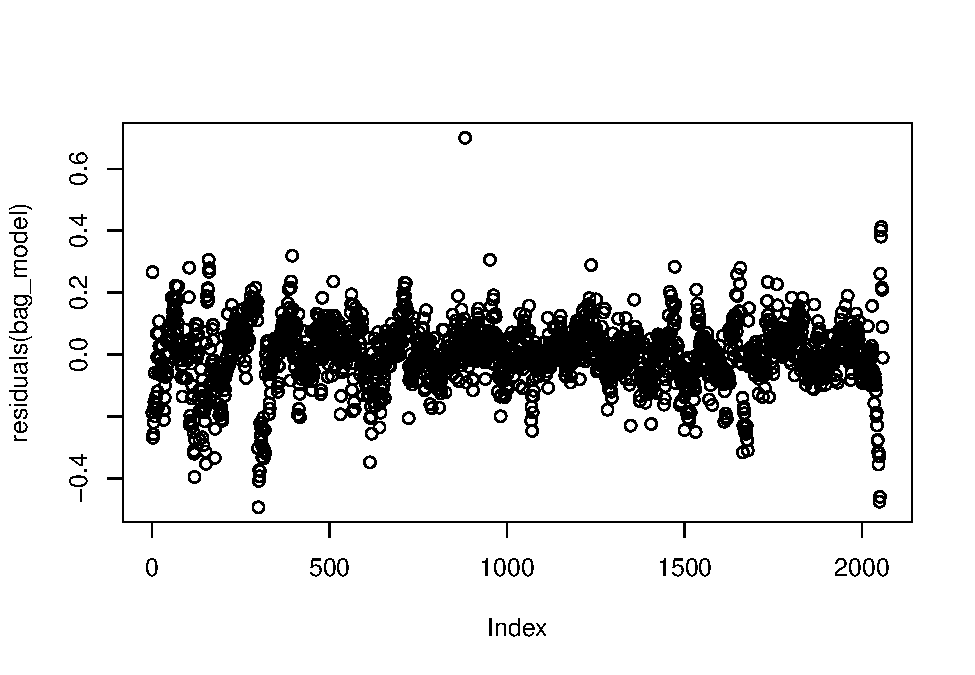
\includegraphics{OmerOzeren_GracieHan_Project_2_files/figure-latex/unnamed-chunk-18-1} \end{center}

\begin{center}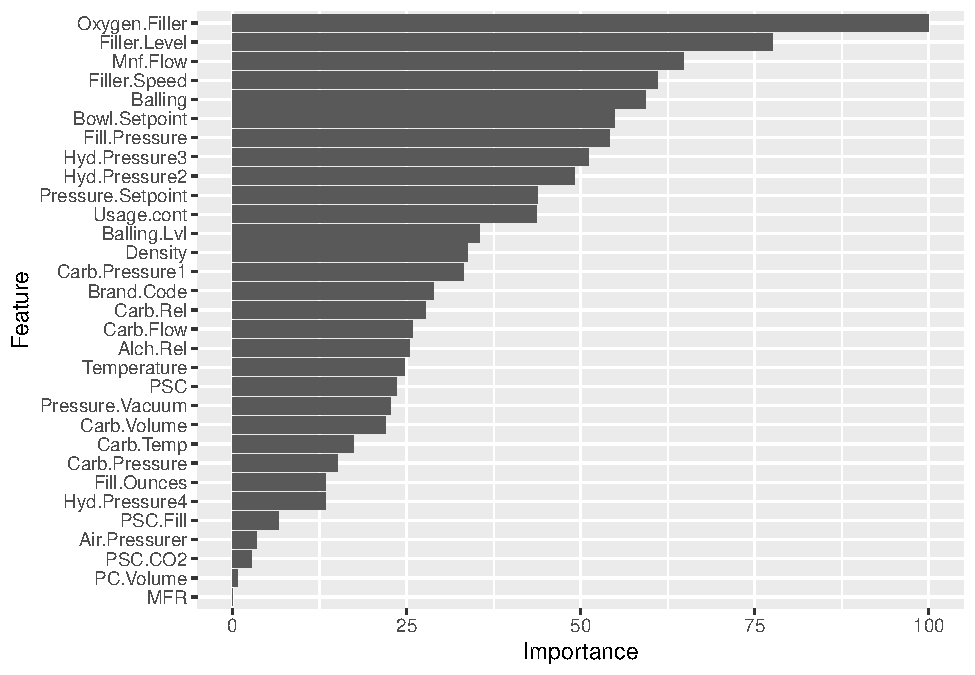
\includegraphics{OmerOzeren_GracieHan_Project_2_files/figure-latex/unnamed-chunk-18-2} \end{center}

First tree based models We selected in is bagged tree model. Each Model
in the bagged tree ensemble is used to generate a prediction for a new
sample and these M predictions are averaged to give the bag to models
prediction. Two steps Algorithms are used, First upon bootstrapling
sample of the original data is generated; Second step, pruning of the
tree model is produced. This algorithm applies from first to the mth
(from 1 to M) observations, and then repeated so on so forth.

Compared with linear regression model, backing also has another
advantage, where they provide their own internal estimate of performance
with cross validation. In our model, we Chose five bootstrap samples for
each algorithem, and then fit 10 Cross valication, with 25 tuning
algorithms.

We chose not to print the evaluation, rather we we will produce summary
data set which contains this model evaluation side-by-side at the end.

Because bagged bootstrapping is an computationally really expensive
process, the run time yes about 5 to 10 times longer compared to the
linear model.

\subsubsection{SVM Model}\label{svm-model}

\begin{center}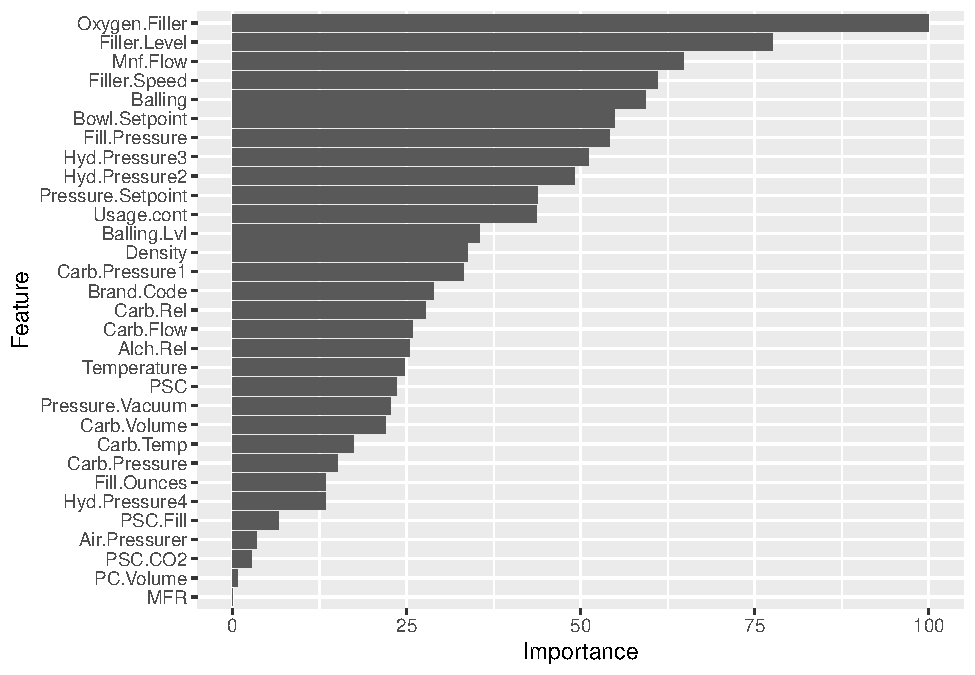
\includegraphics{OmerOzeren_GracieHan_Project_2_files/figure-latex/unnamed-chunk-19-1} \end{center}

Support vector machine algorithm has some advantage over linear
regression in that it minimize the effect of outliers.

In linear regression even one outlier can influence parameter
estimation, but SVM uses the Square to residuals when the abosulte
outliers are small while uses the absolute residuals when the absolute
residuals are large. By this ``weighted effect'', the mangitude of
outlier influence is minimized.

Because our data contains quite a few outliers in a few of the
observations ,we expect that SVM will give us a more robust prediction
than linear model.

\subsubsection{KNN Model}\label{knn-model}

\begin{center}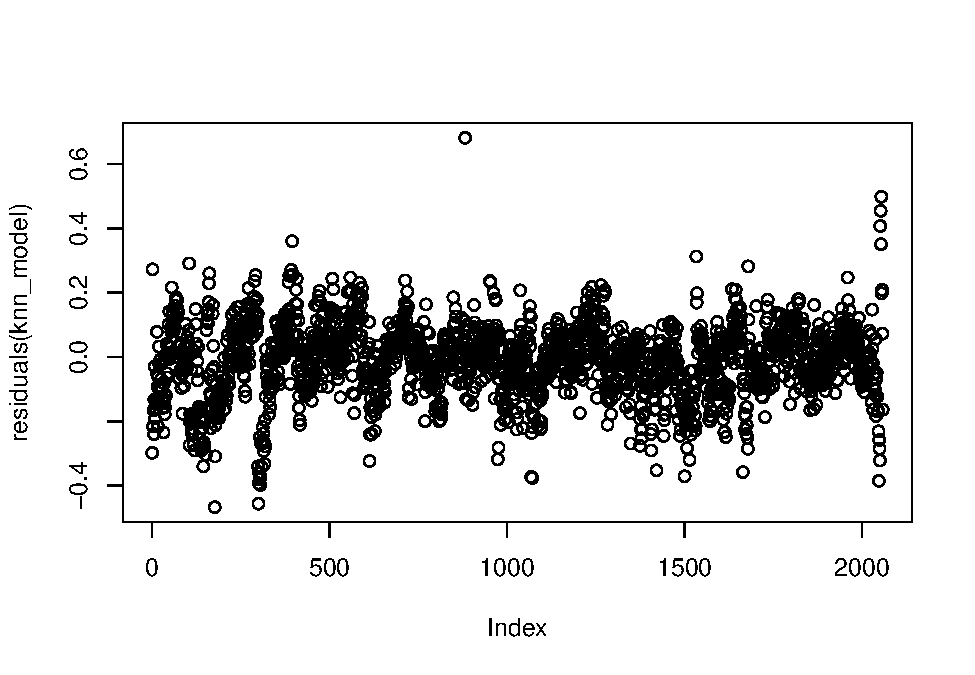
\includegraphics{OmerOzeren_GracieHan_Project_2_files/figure-latex/unnamed-chunk-20-1} \end{center}

\begin{center}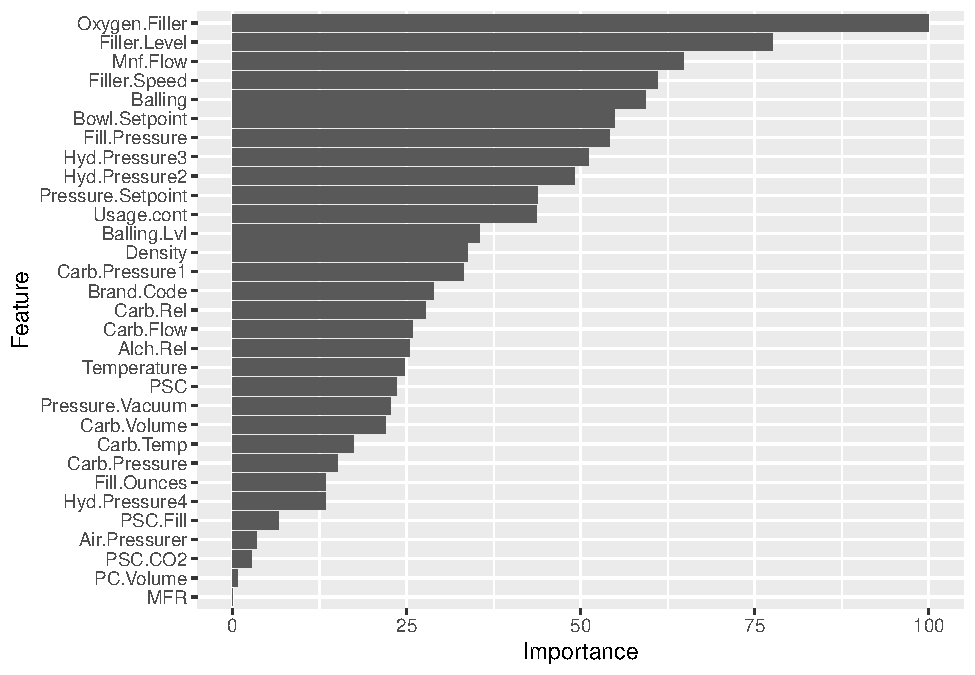
\includegraphics{OmerOzeren_GracieHan_Project_2_files/figure-latex/unnamed-chunk-20-2} \end{center}

KNN, which stands for K nearest neighbors model, utilizes the K closest
samples (Usually in means)from the training set to predict. Its
prediction power can be negatively influenced by different skills of
predictions, which generates unbalanced distance. Because the 33
variables of ours have such issue, we utilized the Options of centered
and scaled predictors to overcome this issue.

As with other model, 10 folds of cross validation were chosen, and 25
tuning algorithm within the KNN modeling were specified. The models
evaluation were bind into the models\_test\_evaluation data frame, to
compared with other models.

\subsubsection{Random Forest}\label{random-forest}

Random forest is one step further of the bagged tree model, but it
differs from the simple bagged tree samples that it completely removes
the inter-dependency of bootstrap samples from regular tree models. It
reduces the correlation among predictors by and adding randomness to the
construction process, hence with the name random forest.

As with other models, we specified 10 cross validations, 25 tuning
algorithms, and we export the model evaluators for future comparisons.

\subsubsection{Cubist Model}\label{cubist-model}

\begin{center}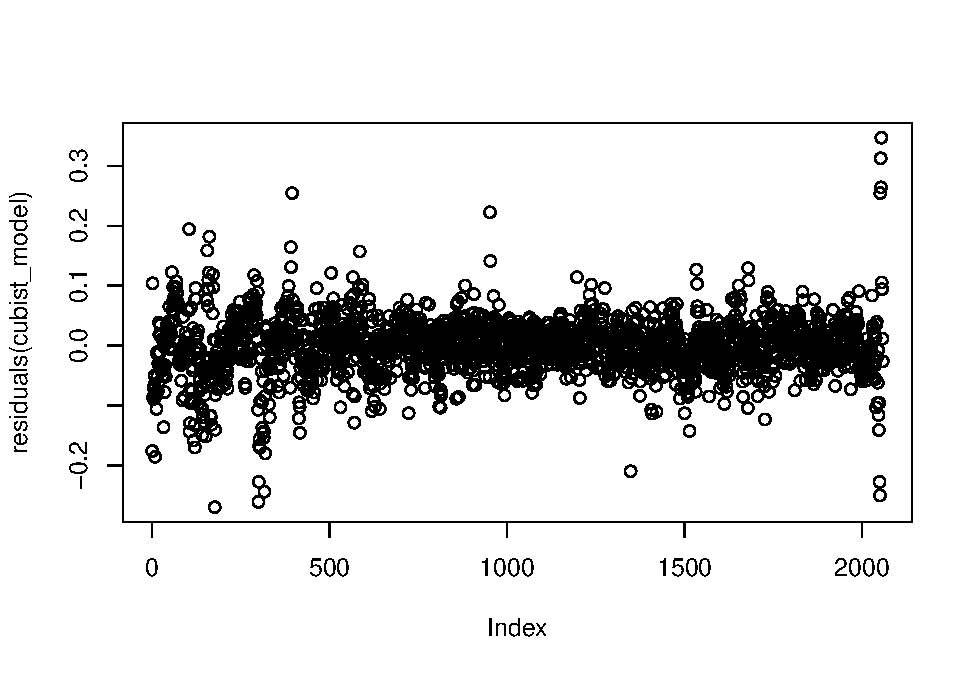
\includegraphics{OmerOzeren_GracieHan_Project_2_files/figure-latex/unnamed-chunk-22-1} \end{center}

\begin{center}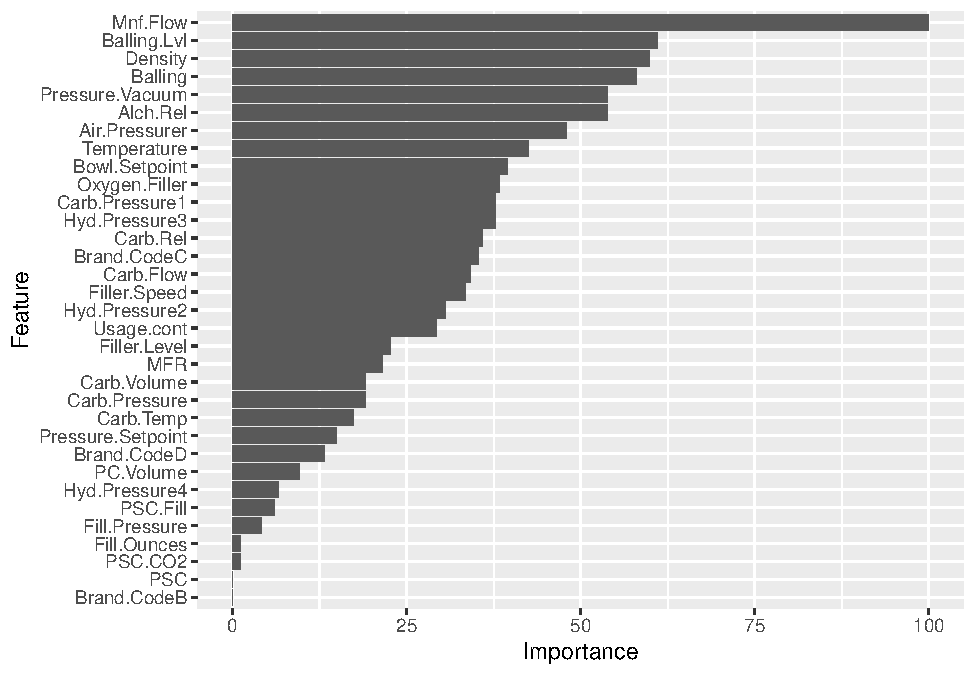
\includegraphics{OmerOzeren_GracieHan_Project_2_files/figure-latex/unnamed-chunk-22-2} \end{center}

Cubist is a rule-based machine learning model. A rule based machine
learner has one step further than the tree based modeling, in that is
the identification and utilization of a set of relational rules that
collectively represent the knowledge. In contrast to Tree based models,
Which generate machine learning rule (also only SINGLE set of rule is
applied) within it self, or in other case, uses only one rule
universally across all the algorithms.

A cute best model resembles a piecewise linear model to predict numeric
values, except that the rules can overlap.

Here, we did the 10 cross validation within each ensemble, with 25
tuning lens length. Then Store the RMS and other evaluators for print
out later, and store them into the models\_test\_evaluation data frame
as a row.

\subsubsection{Multivariate Adaptive Regression Splines
(MARS)}\label{multivariate-adaptive-regression-splines-mars}

\begin{center}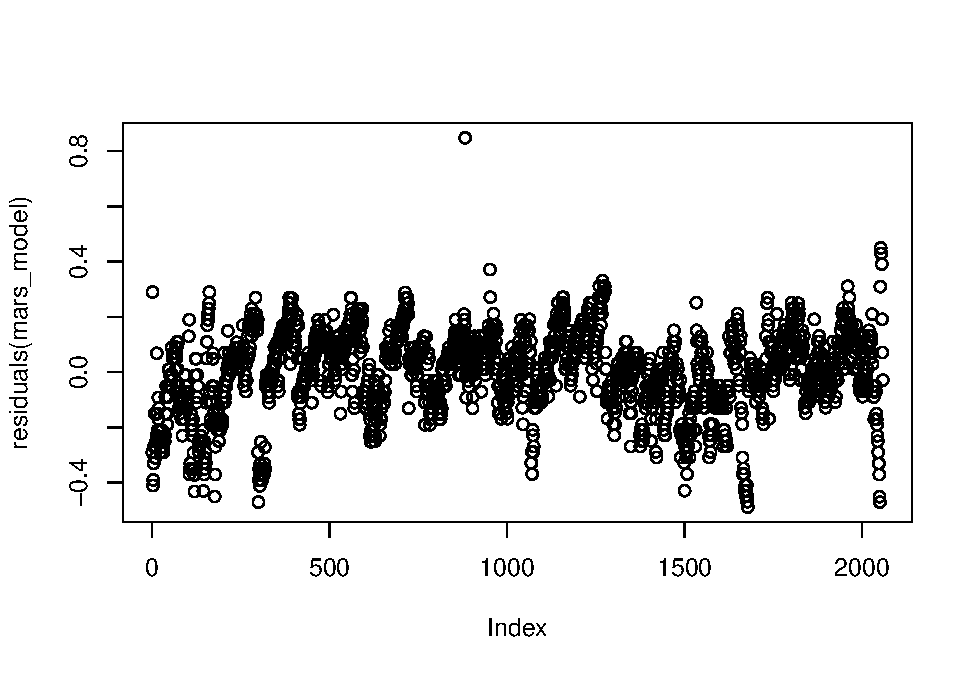
\includegraphics{OmerOzeren_GracieHan_Project_2_files/figure-latex/unnamed-chunk-23-1} \end{center}

\begin{center}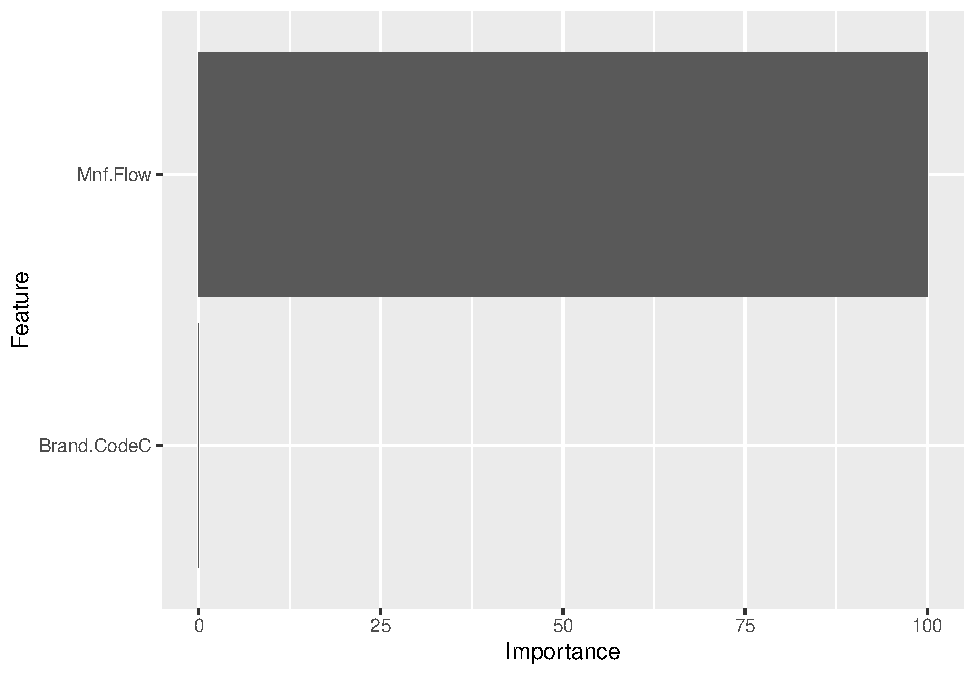
\includegraphics{OmerOzeren_GracieHan_Project_2_files/figure-latex/unnamed-chunk-23-2} \end{center}

Due to the strict assumption of linearity between predictors and
outcome, problem arise when multiple variables, in our case, 33
predictors are in presence, many of whom do not have the perfect linear
relationship with the outcome. Such problem might be solved by
introducing some nonlinearity in the model, such as to supplement the
previous linear regression model with additional complexity. Adding a
squared term, or even higher dimensional term, for some variables, or
introducing interaction term with two correlated variables. But the
model can be overly complex by such, which introduces many more
unnecessary variables in addition to the existing 33 variables, which
exacerbates the overfitting problem even further.

The multivariate adaptive regression spline (MARS) model is a solution
to such dilemma. When used with a single predictor, MARS can fit
separate linear regression lines for different ranges of engine
displacement. The slopes and intercepts are estimated for this model, as
well as the number and size of the separate regions for the linear
models.

\subsection{Model Evalution Summary}\label{model-evalution-summary}

\begin{verbatim}
##           Model       RMSE  Rsquared        MAE
## 1          MARS 0.14542857 0.3143190 0.11438384
## 2        Cubist 0.09207475 0.7254765 0.06671164
## 3 Random Forest 0.09390085 0.7291957 0.06885157
## 4          KNN  0.11969112 0.5419179 0.09081871
## 5           SVM 0.11525275 0.5719417 0.08339187
## 6  Bagged-Tree  0.11029114 0.6086628 0.08150475
\end{verbatim}

The table above shows our models performance.We evaluated models using
below criteria:

\begin{enumerate}
\def\labelenumi{\arabic{enumi}.}
\tightlist
\item
  R\^{}2
\end{enumerate}

Overall, Except the MARS model (R\^{}2=0.27), the R squared are Within
the range of 0.50 to 0.69 for all the tree based and rule based models.

Remember that the R squared in Linear model is 0.42(multiple R squared),
and 0.4081(adjusted R squares), the lower R\^{}2of MARS indicates that
it is an inferior model to linear model.

The rest of five models have shown improvement in R-squared compared to
the linear model. The improvements are most robust in random forest
model (0.69 R squared, or 50\% improvement from the linear model,), and
the cubist model model (R-square 0.676, also 50\% improvement from the
linear model as well). The KNN and the SVM, bagged tree Model have
R-squared around 0.53, not a significant improvement from linear model
in terms of R squared.

\begin{enumerate}
\def\labelenumi{\arabic{enumi}.}
\setcounter{enumi}{1}
\tightlist
\item
  \emph{Root Mean Squared Error}
\end{enumerate}

RMSE is interpreted as how far, on average, the residuals are from zero.

The RMSE is lowest in Cubist model (RMSE=0.10) and in random forest
model (RMSE=0.101). The MARS have the worst performance in terms of RMSE
(RMSE=0.15).The rest of 3 tree based models (KNN, SVM, bagged tree) have
similar RMSE at 0.12.

\begin{enumerate}
\def\labelenumi{\arabic{enumi}.}
\setcounter{enumi}{2}
\tightlist
\item
  \emph{Mean Absolute Error} (MAE)
\end{enumerate}

The MAE value follows exactly the same pattern as RMSE. The best the
performers are cubist, random forest model. While the worst performer is
MARS. The rest of three models perform similarly.

Based on what we've seen above table Cubist model gives best performance
among the other models.So we are going to select Cubist models as
champion model and predict values by using evaluation dataset and export
in excel file.

Taking into all considerations of RMSE, R squared, MAE, Cubist is our
best model. Random forest model follows very closely to Cubist.

The linear model and the MARS, multi-adaptive regression sblinds model
clearly do not have much advantage in predicting PH from these 33
variables.

\end{document}
